\documentclass[a4paper, twoside, english]{article}

\usepackage{amsmath}
\usepackage{amsfonts}
\usepackage{ihci}
\usepackage{graphicx}
\usepackage{subfig}

\graphicspath{{./../figures/}}

\title{Exercise 1 - Theory}
\author{
	Abdelaziz, Ibrahim
	\and
	Somkiadcharoen, Robroo
	\and
	Berg, Oliver
}
\date{\today}

\begin{document}
\maketitle


\section{Properties of Rotation Matrices}

\subsection{Showing that $U^T = U^{-1}$ holds for \textit{general} rotation matrix $U \in \mathbb{R}^3$}

Generally note that $UU^{-1}=I$ subject to $U^{-1} = U^T$, as provided by $U$ being rotation matrix and as such orthogonal, yields $UU^T = I$.

For given column-vectors $c_1, c_2, c_3$ of $U$ we observe 

\begin{equation*}
	<c_i, c_j> = \delta_{i j}
\end{equation*}

which in combination with

\begin{equation*}
	U^T = (c_1, c_2, c_3)^T = (c_1^T, c_2^T, c_2^T)
\end{equation*}

results in

\begin{equation*}
	UU^T = (<c_i, c_j>)_{1 \le i, j \le 3} = I
\end{equation*}

Motivated by \cite{MathematicsSEMatrixTransposeIdentity}\cite{MathematicsSEMatrixTransposeIdentity2}\cite{WikiOrthogonaleMatrix}.

\subsection{Geometric interpretation of determinant of 3x3 matrix}

The determinant of a matrix $A \in \mathbb{R}^3$ has the geometric intuition of a scaling factor for a given (unit) volume within the cartesian (standard) coordinate system and how its volume changes when applying the matrix transform. \cite{3blue1brownLinAlg5Determinant}

As such, with $det(A) = 1$ the matrix does not change the size of any given volume within its space, which intuitively makes sense for a rotation matrices as its only task is to rotate - not scale - within any given coordinate system.


\section{Transformation Chain}

Normally, the transformation mapping from the world coordinate system to pixel coordinate system is.

\begin{equation*}
	\begin{bmatrix}
		u' \\
		v' \\
		w'
	\end{bmatrix} = K[I_3| O_3]
	\begin{bmatrix}
	R & T \\
	0_3^T & 1
	\end{bmatrix}
	\begin{bmatrix}
	X_s \\
	Y_s \\
	Z_s \\
	1
	\end{bmatrix}
\end{equation*}


Where $x_{pix}$ and $y_{pix}$ are $u'/w'$ and $v'/w'$ 
and $
\begin{bmatrix}
	X_s & Y_s & Z_s & 1
\end{bmatrix}^T 
$ are the coordinates of a 3D point in the world coordinate space

Homogeneous Coordinates is good. It enables us to use Matrix Multiplication on all transformations. To represent 3d coordinate points you need to have 4 elements in the vector.
\begin{equation}
[x,y,z,w] = [x/w,y/w,z/w]
\end{equation}
However, when $w$ in $(1)$ is $0$. There is no such 3D vector on that. We call points in this form vanishing point.\cite{TheTruthBehindHomoCoords}

\subsection{Chain Step}
\begin{equation*}
\begin{bmatrix}
x_s \\
y_s \\
z_s \\
1
\end{bmatrix}
=
\begin{bmatrix}
	R & T \\
	0_3^T & 1
\end{bmatrix}
\begin{bmatrix}
	X_s \\
	Y_s \\
	Z_s \\
	1
\end{bmatrix}
\end{equation*}
multiplying $\begin{bmatrix}
R & T \\
0_3^T & 1
\end{bmatrix}$ to the world coordinates $[X_s,Y_s,Z_s,1]^T$ gives a camera coordinates $[x_s,y_s,z_s,1]^T$

\begin{equation*}
\begin{bmatrix}
u' \\
v' \\
w'
\end{bmatrix}
=
\begin{bmatrix}
a_x & s & x_0 & 0 \\
0 & a_y & y_0 & 0\\
0 & 0 & 1 & 0
\end{bmatrix}
\begin{bmatrix}
x_s \\
y_s \\
z_s \\
1
\end{bmatrix}
\end{equation*}
By multiplying the camera coordinate points with calibration matrix, the result is in the image plane coordinates. After that we can do $u'/w'$ and $v'/w'$ to get the pixel coordinates

\subsection{Intrinsic parameters}

$K$ is a camera matrix, or a matrix of intrinsic parameters $K=\begin{bmatrix}
a_x & s & x_0  \\
0 & a_y & y_0 \\
0 & 0 & 1
\end{bmatrix}$ 
Where \begin{itemize}
	\item $a_x$ and $a_y$ are focal lengths in pixel 
	\item $x_0$ and $y_0$ are the image center
	\item $s$ the skew coefficient between the x,y axis which is 0 in most cases \cite{CameraResectioning}\cite{OpenCVDocCameraCalib}
\end{itemize}
$K$ can transform image plane to pixels and $\begin{bmatrix}
I_3 &|& O_3 
\end{bmatrix}
=
\begin{bmatrix}
1 & 0 & 0 & 0 \\
0 & 1 & 0 & 0 \\
0 & 0 & 1 & 0
\end{bmatrix}$ can be use for perspective projection which can be combined to K matrix and facilitate the matrix multiplication



\subsection{Extrinsic parameters}
\begin{equation*} extrinsicParams = 
\begin{bmatrix}
R & T \\
0_3^T & 1
\end{bmatrix}
\end{equation*}

This extrinsic parameters is used to explain the camera motion along the scene. It translates world-coordinates of a point $[X,Y,Z,1]$ to a camera coordinate system

\begin{equation*} R = 
\begin{bmatrix}
I_i & J_i & K_i \\
I_j & J_j & K_j \\
I_k & J_k & K_k 
\end{bmatrix}
T=
\begin{bmatrix}
T_x \\
T_y \\
T_z
\end{bmatrix}
\end{equation*}
$R$ is a rotational matrix such that it helps rotating the point from world to camera.
$T$ is a translational metric to translate the point from world to camera.
Motivated from \cite{SomeLinearAlgebra}


\section{Implementation}

The final implementation task can be found in \lstinline{main.py}.

Concerning output (images in \textit{output} directory), projected points without correction of distortion are shown in red, those with correction of radial distortion in green; see \autoref{fig:sampleOutputImg}.

\begin{figure}
  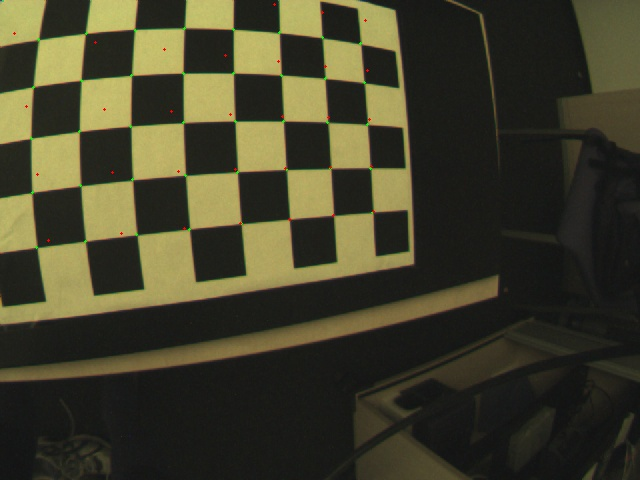
\includegraphics[width=\textwidth]{00000.jpg}
  \caption{Sample output image\label{fig:sampleOutputImg}}
\end{figure}

\bibliographystyle{IEEEtran}
\bibliography{bibliography.bib}
\end{document}